% !TeX program = pdflatex
% Parte V de la serie godsil-gutman-lean (version en espanol).
% Contar arboles sin enumerarlos — una demostracion verificada por maquina del
% teorema matricial de los arboles de Kirchhoff en Lean 4.
% Compilar: pdflatex matrix-tree-lean-es.tex  (dos veces, por las referencias)
% Verificado contra el fuente Lean el 2026-06-10 (lake build, 3074 trabajos, exit 0;
% #print axioms SimpleGraph.det_reducedLapMatrix_eq_card_spanningTrees ->
% propext, Classical.choice, Quot.sound unicamente). Toolchain v4.30.0-rc2, Mathlib local.

\documentclass[11pt]{article}
\usepackage[T1]{fontenc}
\usepackage[utf8]{inputenc}
\usepackage[spanish,es-noshorthands]{babel}
\usepackage{lmodern}
\usepackage{amsmath,amssymb,amsthm,booktabs,graphicx,hyperref}
\usepackage{xurl}
\usepackage[table]{xcolor}
\definecolor{ggteal}{HTML}{1B6F8C}
\definecolor{ggband}{HTML}{DCE7EB}
\definecolor{ggamber}{HTML}{E08A1E}
\usepackage[margin=1in]{geometry}
\usepackage{microtype}
\usepackage[most]{tcolorbox}
\usepackage{tikz}
\usetikzlibrary{arrows.meta,positioning}
\setlength{\emergencystretch}{2em}
\graphicspath{{figures/}}
\newtheorem{theorem}{Teorema}
\newtheorem{lemma}{Lema}
\newtheorem{definition}{Definici\'on}
\newcommand{\lean}[1]{\texttt{#1}}
\newcommand{\Z}{\mathbb{Z}}
\newcommand{\R}{\mathbb{R}}
\newcommand{\N}{\mathbb{N}}
\DeclareMathOperator{\dist}{dist}
\hypersetup{colorlinks=true,linkcolor=ggteal,citecolor=ggteal,urlcolor=ggteal}
\newtcbox{\keybox}{on line,boxrule=0.9pt,colframe=ggteal,colback=ggband!40,
  arc=3pt,left=8pt,right=8pt,top=5pt,bottom=5pt}
\newcommand{\keyeq}[1]{\begin{center}\keybox{$\displaystyle #1$}\end{center}}

\title{\bf Contar \'arboles sin enumerarlos\\[4pt]
  \large\normalfont Una demostraci\'on verificada por m\'aquina del teorema matricial de los
  \'arboles de Kirchhoff en Lean~4}
\author{Carles Mar\'in\thanks{Formalizado con asistencia de IA (Claude, Anthropic); las
matem\'aticas y todas las afirmaciones son responsabilidad del autor. La metodolog\'ia se
discute en la Secci\'on~\ref{sec:implications}.}\\[3pt]
  \normalsize Investigador independiente\\
  \normalsize \texttt{karlesmarin@gmail.com}}
\date{Junio de 2026}

\begin{document}
\maketitle

\begin{abstract}
Presento una demostraci\'on verificada por m\'aquina, libre de \lean{sorry}, en Lean~4 sobre
Mathlib, del \emph{teorema matricial de los \'arboles} de Kirchhoff: sobre cualquier dominio
\'integro, el determinante del laplaciano reducido de un grafo simple finito es igual a su
n\'umero de \'arboles generadores. La demostraci\'on se arma con cuatro piezas formalizadas,
cada una \'util por s\'i misma: la f\'ormula de Cauchy--Binet para el determinante
$\det(AB)$ de un par rectangular; la matriz de incidencia \emph{orientada} y su factorizaci\'on
de Gram $NN^{\mathsf T}=D-A$ (Mathlib solo dispone de la incidencia sin orientar, cuya matriz
de Gram es $D+A$); la expansi\'on por Cauchy--Binet del determinante del laplaciano reducido en
una suma de menores maximales al cuadrado; y un teorema de dicotom\'ia que identifica ese
cuadrado como $1$ exactamente sobre los conjuntos de aristas de los \'arboles generadores y $0$
en el resto. La dicotom\'ia se demuestra \emph{sin} la inducci\'on por poda de hojas de los
libros de texto: a cada v\'ertice distinto de la ra\'iz de un subgrafo conexo se le asigna su
\emph{arista padre} sobre una geod\'esica hacia la ra\'iz, el menor as\'i re-columnado resulta
triangular superior bajo la clave lexicogr\'afica $(\text{distancia a la ra\'iz},\,
\text{v\'ertice})$, y el determinante es el producto de su diagonal de $\pm1$. Un subproducto
del dise\~no es que nunca llega a construirse un argumento separado de aciclicidad: la
conexi\'on y el conteo de aristas---que juntos, cl\'asicamente, ya caracterizan los
\'arboles---son las \'unicas entradas que consume la demostraci\'on formal. El teorema principal depende \'unicamente de los tres axiomas est\'andar. Soy
exacto con la frontera: el resultado vale para grafos simples finitos sobre un dominio
\'integro; el polinomio de Kirchhoff con pesos, el teorema de todos los menores y la versi\'on
dirigida quedan cartografiados pero no construidos; existe una formalizaci\'on independiente de
Cauchy--Binet en Lean (no en Mathlib), surgida en el proyecto del libro de Grinberg, que se
discute en la Secci\'on~\ref{sec:boundary}; del teorema matricial de los \'arboles en s\'i no
he logrado localizar formalizaci\'on previa en ning\'un asistente de demostraci\'on, aunque una
afirmaci\'on as\'i solo puede hacerse hasta donde alcanza el conocimiento de uno.
\end{abstract}

\noindent\emph{Mapa del lector.} Si lee una sola cosa, lea el Teorema~\ref{thm:kirchhoff} y la
Figura~\ref{fig:triangular}: el enunciado, y el dibujo de por qu\'e el menor de un \'arbol
generador vale $\pm1$. La demostraci\'on es una sola cadena (Figura~\ref{fig:road}); cada
eslab\'on tiene su secci\'on, su figura y un ejemplo lo bastante peque\~no para comprobarlo a
mano. Los l\'imites honestos est\'an en la Secci\'on~\ref{sec:boundary}.

% ---------------------------------------------------------------
\section{Introducci\'on: dos memorias y un circuito}
\label{sec:intro}

El 30 de noviembre de 1812 se leyeron en el Institut de France, el mismo d\'ia, dos memorias
sobre determinantes: una de Jacques Binet, otra de Augustin-Louis
Cauchy~\cite{Binet1812,Cauchy1812}. Ambas conten\'ian, entre mucho m\'as, la f\'ormula que hoy
lleva los dos nombres: el determinante del producto de dos matrices rectangulares es una suma,
sobre todas las maneras de recortar un cuadrado de la dimensi\'on compartida, de productos de
menores correspondientes. Es el teorema m\'as antiguo de este art\'iculo, y su ingrediente m\'as
profundo.

Treinta y cinco a\~nos despu\'es, Gustav Kirchhoff no estudiaba determinantes. Estudiaba
circuitos el\'ectricos---las ecuaciones lineales que gobiernan las corrientes en una red de
resistencias~\cite{Kirchhoff1847}---y encontr\'o que la cantidad que controla su resolubilidad
cuenta algo puramente combinatorio: los \'arboles generadores del grafo de la red. En lenguaje
moderno, con $D$ la diagonal de grados y $A$ la matriz de adyacencia, el \emph{laplaciano}
$L=D-A$ de un grafo $G$ con $n$ v\'ertices es singular (sus filas suman cero), pero al tachar
una fila cualquiera y su columna queda una matriz $L_0$ de orden $(n-1)$ con
\[
  \det L_0 \;=\; \tau(G),
\]
el n\'umero de \'arboles generadores de $G$---sea cual sea la fila tachada. Un determinante
computable en tiempo polin\'omico cuenta una familia t\'ipicamente exponencial; la matriz sabe
la respuesta sin que nadie haya listado un solo \'arbol.

El teorema llev\'o despu\'es una doble vida. Borchardt dio la primera demostraci\'on
determinantal en 1860~\cite{Borchardt1860}; la c\'elebre cuenta $n^{n-2}$ de Cayley para los
\'arboles etiquetados, en una nota breve de 1889, es la f\'ormula evaluada en el grafo
completo~\cite{Cayley1889}. En 1940, Brooks, Smith, Stone y Tutte diseccionaron rect\'angulos
en cuadrados interpretando la disecci\'on como una corriente que fluye por una red
plana---los circuitos de Kirchhoff regresando a las matem\'aticas~\cite{BSST1940}. Tutte
extendi\'o la cuenta a grafos dirigidos y arborescencias~\cite{Tutte1948}; Chaiken y Kleitman
probaron la generalizaci\'on de todos los menores~\cite{ChaikenKleitman1978,Chaiken1982}. En la
probabilidad moderna el teorema es estructural: el algoritmo de Wilson muestrea un \'arbol
generador uniforme m\'as r\'apido que el tiempo de cubrimiento~\cite{Wilson1996}, el teorema de
las corrientes de transferencia convierte el \'arbol generador uniforme en un proceso
determinantal~\cite{BurtonPemantle1993}, y las resistencias efectivas---cocientes de cuentas de
\'arboles---impulsan la dispersi\'on espectral de grafos~\cite{SpielmanSrivastava2011}. Las
referencias cl\'asicas son~\cite{Moon1970,Biggs1993,GodsilRoyle,StanleyEC2,LyonsPeres}.

Lo que el teorema no ten\'ia, hasta donde he podido encontrar, es una demostraci\'on verificada
por m\'aquina. La biblioteca matem\'atica de Lean~\cite{Mathlib} dispone del laplaciano y conoce
su n\'ucleo; dispone de la matriz de incidencia \emph{sin orientar}; y gan\'o hace poco, en un
proyecto independiente de formalizaci\'on de un libro de texto, la f\'ormula de
Cauchy--Binet~\cite{Grinberg,FaabianRepo}---pero no el teorema matricial de los \'arboles, del
que tampoco encontr\'e formalizaci\'on en el Archive of Formal Proofs de Isabelle ni en el
ecosistema Coq/Rocq. Este art\'iculo cierra ese hueco, como Parte~V de una serie que formaliza
el c\'irculo de ideas paseos--emparejamientos--espectro alrededor del polinomio de
emparejamientos~\cite{PartI,PartII,Bass,PartIII,PartIV}.

Una cosa m\'as, y es el giro que deja escrito este art\'iculo. Toda demostraci\'on de libro de
texto de la dicotom\'ia que sostiene el teorema---\emph{un conjunto de $n-1$ aristas tiene menor
$\pm1$ si es un \'arbol generador y $0$ si no}---poda una hoja e induce. La demostraci\'on
formal hace algo con lo que una m\'aquina est\'a mucho m\'as c\'omoda: \emph{ordena}. Cada
v\'ertice distinto de la ra\'iz se empareja con su \emph{arista padre} sobre una geod\'esica
hacia la ra\'iz; ordenar los v\'ertices por distancia vuelve el menor triangular superior con
diagonal $\pm1$, y el determinante cae como un producto (Figura~\ref{fig:triangular}). Sin
inducci\'on sobre grafos en ninguna parte. Y una observaci\'on menor, de ingenier\'ia de
demostraciones m\'as que de matem\'aticas: de las dos mitades de la caracterizaci\'on de
\'arbol ((conexo y ac\'iclico con $n-1$ aristas)), la demostraci\'on formal solo consume la
conexi\'on m\'as el conteo---la mitad ac\'iclica equivalente, aunque por supuesto implicada,
nunca llega a materializarse como lema. A la m\'aquina nunca se le pide buscar un ciclo.

% ---------------------------------------------------------------
\section{El resultado}
\label{sec:result}

En todo el art\'iculo, $G$ es un grafo simple finito sobre un tipo de v\'ertices $V$ con un
orden lineal (cualquier enumeraci\'on de los v\'ertices), $v_0\in V$ una \emph{ra\'iz} fija, y
$R$ un anillo conmutativo---un dominio \'integro donde se indique. Escribimos $n=|V|$. El
enunciado Lean del teorema principal es:

\begin{theorem}[{\lean{SimpleGraph.det\_reducedLapMatrix\_eq\_card\_spanningTrees}}]
\label{thm:kirchhoff}
Sea $R$ un dominio \'integro. Entonces
\keyeq{\det L_0 \;=\; \#\Bigl\{\,S\subseteq\mathrm{Sym}^2 V \;:\; |S|=n-1,\;
S\subseteq E(G),\; (V,S)\ \text{es un \'arbol}\,\Bigr\}}
donde $L_0$ es el laplaciano de $G$ sin la fila ni la columna de $v_0$, y la cuenta se
inyecta en $R$.
\end{theorem}

En Lean, el lado derecho es un \lean{Finset.filter} sobre el subtipo de los subconjuntos de
\lean{Sym2 V} con $n-1$ elementos, con la condici\'on
$\uparrow\!S\subseteq G.\lean{edgeSet}\;\wedge\;(\lean{fromEdgeSet}\ \uparrow\!S).\lean{IsTree}$;
como \lean{fromEdgeSet} coloca el subgrafo sobre \emph{todo} $V$, \lean{IsTree} ya incorpora
que sea generador. Todo \'arbol generador de $G$ tiene exactamente $n-1$ aristas y queda
determinado por su conjunto de aristas, de modo que el filtro cuenta \'arboles generadores,
cada uno exactamente una vez.

\begin{figure}[t]
  \centering
  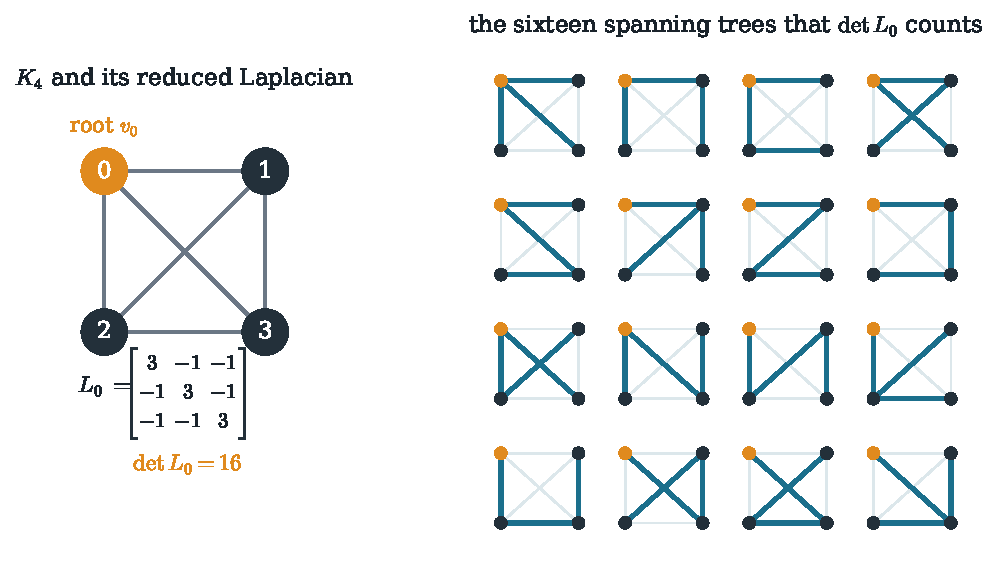
\includegraphics[width=0.96\textwidth]{mt_fig1_k4trees}
  \caption{El teorema sobre $K_4$, con ra\'iz $v_0$. El laplaciano reducido es la matriz
  $3\times3$ de la izquierda; su determinante vale $16$, y a la derecha est\'an los diecis\'eis
  \'arboles generadores que cuenta. La f\'ormula de Cayley $n^{n-2}$ da $4^2=16$; el
  determinante llega al mismo n\'umero sin enumerar nada.}
  \label{fig:k4}
\end{figure}

?`Para qu\'e sirve el teorema? Convierte una enumeraci\'on exponencial en un c\'alculo de
\'algebra lineal en tiempo polin\'omico. El grafo de Petersen tiene $2000$ \'arboles
generadores; nadie los encuentra list\'andolos. Se escribe el laplaciano reducido, de orden
$9\times9$, y se toma un determinante. El mismo intercambio alimenta todo lo de la
Secci\'on~\ref{sec:implications}: cuentas de fiabilidad, muestreo uniforme, resistencias
efectivas. La Tabla~\ref{tab:numbers} muestra el teorema en acci\'on sobre seis grafos
cl\'asicos, con ambos lados calculados de forma independiente en SageMath.

\begin{table}[h]
\centering
\rowcolors{2}{ggband!35}{white}
\begin{tabular}{lccc}
\toprule
\rowcolor{ggteal!18} grafo & $n$ & $\det L_0$ & $\tau(G)$ (cuenta independiente) \\
\midrule
$K_4$          & 4  & 16   & 16   \\
$K_5$          & 5  & 125  & 125  \\
$C_6$ (ciclo)  & 6  & 6    & 6    \\
$K_{3,3}$      & 6  & 81   & 81   \\
$Q_3$ (cubo)   & 8  & 384  & 384  \\
Petersen       & 10 & 2000 & 2000 \\
\bottomrule
\end{tabular}
\caption{Los dos lados del Teorema~\ref{thm:kirchhoff} calculados de forma independiente
(SageMath, aritm\'etica entera exacta). N\'otese que $K_4$ y $K_5$ son los $4^{2}$ y $5^{3}$ de
Cayley; $C_6$ cuenta sus seis maneras de borrar una arista.}
\label{tab:numbers}
\end{table}

% ---------------------------------------------------------------
\section{La cadena, en cuatro eslabones}
\label{sec:chain}

La demostraci\'on formal es una cadena de cuatro resultados, cada uno utilizable por separado.
La Figura~\ref{fig:road} muestra las dependencias; la Tabla~\ref{tab:loadbearing} recoge los
nombres Lean. El relato de las cuatro secciones siguientes no hace m\'as que recorrer la cadena.

\begin{figure}[h]
\centering
\begin{tikzpicture}[
  stone/.style={draw=ggteal,fill=ggband!40,rounded corners=3pt,align=center,
    inner sep=6pt,font=\small},
  final/.style={draw=ggamber,fill=ggamber!12,rounded corners=3pt,align=center,
    inner sep=6pt,font=\small\bfseries},
  arr/.style={-{Stealth[length=2.4mm]},thick,ggteal}]
  \node[stone] (cb) at (0,2.1) {Cauchy--Binet (1812)\\
    $\det(AB)=\sum_S \det A_S\,\det B_S$\\ \S\ref{sec:cb}};
  \node[stone] (gram) at (0,0) {incidencia orientada\\
    $NN^{\mathsf T}=D-A$\\ \S\ref{sec:gram}};
  \node[stone] (sum) at (5.6,1.05) {expansi\'on reducida\\
    $\det L_0=\sum_S(\det N_{0,S})^2$\\ \S\ref{sec:sum}};
  \node[stone] (dich) at (5.6,-1.2) {dicotom\'ia\\
    $(\det N_{0,S})^2=\mathbb 1[S\ \text{genera un \'arbol}]$\\ \S\ref{sec:dichotomy}};
  \node[final] (kir) at (11.0,0) {Kirchhoff\\ $\det L_0=\tau(G)$\\
    Teor.~\ref{thm:kirchhoff}};
  \draw[arr] (cb) -- (sum);
  \draw[arr] (gram) -- (sum);
  \draw[arr] (sum) -- (kir);
  \draw[arr] (dich) -- (kir);
  \draw[arr] (gram) -- (dich);
\end{tikzpicture}
\caption{La cadena de la demostraci\'on. Dos ingredientes cl\'asicos se combinan en la
expansi\'on como suma de cuadrados; la dicotom\'ia decide cada sumando; la cuenta cae sola.}
\label{fig:road}
\end{figure}

\begin{table}[h]
\centering\footnotesize
\rowcolors{2}{ggband!35}{white}
\begin{tabular}{lll}
\toprule
\rowcolor{ggteal!18} teorema Lean & enunciado & fichero (bajo \lean{Ihara/}) \\
\midrule
\lean{det\_mul\_cauchyBinet} & $\det(AB)=\sum_S\det A_S\det B_S$ & \lean{CauchyBinet.lean} \\
\lean{orientedIncMatrix\_mul\_transpose} & $NN^{\mathsf T}=D-A$ & \lean{OrientedIncidence.lean} \\
\lean{det\_reducedLapMatrix\_eq\_sum\_sq} & $\det L_0=\sum_S(\det N_{0,S})^2$ & \lean{MatrixTree.lean} \\
\lean{sq\_det\_minor\_eq\_ite} & $(\det N_{0,S})^2=\mathbb 1[S\ \text{genera \'arbol}]$ & \lean{SpanningTreeMinor.lean} \\
\lean{det\_reducedLapMatrix\_eq\_card\_spanningTrees} & $\det L_0=\tau(G)$ & \lean{Kirchhoff.lean} \\
\bottomrule
\end{tabular}
\caption{Los resultados portantes. Todos libres de \lean{sorry}; cada
\lean{\#print axioms} devuelve exactamente \lean{propext}, \lean{Classical.choice} y
\lean{Quot.sound}.}
\label{tab:loadbearing}
\end{table}

% ---------------------------------------------------------------
\section{Un teorema de 1812}
\label{sec:cb}

\begin{theorem}[{\lean{Matrix.det\_mul\_cauchyBinet}}]
\label{thm:cb}
Sea $R$ un anillo conmutativo, $A$ una matriz $m\times n$ y $B$ una matriz $n\times m$ sobre
$R$. Entonces
\keyeq{\det(AB)\;=\;\sum_{\substack{S\subseteq\{1,\dots,n\}\\ |S|=m}}
  \det A_{\cdot,S}\,\cdot\,\det B_{S,\cdot}}
donde $A_{\cdot,S}$ conserva las columnas de $A$ con \'indice en $S$, en orden creciente, y
$B_{S,\cdot}$ las filas correspondientes de $B$.
\end{theorem}

Si $m>n$ la suma es vac\'ia y el determinante es $0$; si $m=n$ es la multiplicatividad de
$\det$. El caso genuinamente rectangular es el \'util: \emph{toda matriz de Gram es el producto
de una matriz por su traspuesta}, y Cauchy--Binet convierte su determinante en una suma de
cuadrados---no-negatividad gratis sobre los reales y, en este art\'iculo, una suma sobre
conjuntos candidatos de aristas. La Figura~\ref{fig:cb} desarrolla a mano el caso no trivial
m\'as peque\~no.

\begin{figure}[t]
  \centering
  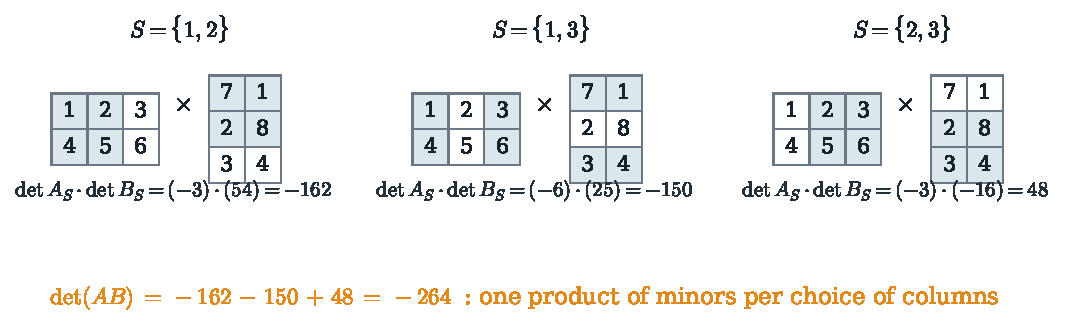
\includegraphics[width=0.98\textwidth]{mt_fig2_cauchybinet}
  \caption{Cauchy--Binet para un producto $2\times3$ por $3\times2$. Tres maneras de elegir dos
  de los tres \'indices intermedios; cada una aporta el producto de los dos menores sombreados.
  Los tres productos $-162-150+48$ suman $\det(AB)=-264$, que se comprueba directamente:
  $AB=\left(\begin{smallmatrix}20&29\\56&80\end{smallmatrix}\right)$.}
  \label{fig:cb}
\end{figure}

La demostraci\'on Lean tiene tres movimientos, y el del medio es donde vive el contenido de la
f\'ormula. \emph{Primero}, expandir $\det(AB)$ por la f\'ormula de Leibniz y distribuir el
producto sobre las sumas del producto matricial da una expansi\'on sobre \emph{todas} las
funciones $g:\{1..m\}\to\{1..n\}$,
\[
  \det(AB)\;=\;\sum_{g}\;\det A_{\cdot,g}\cdot\prod_{i}B_{g(i),i}
  \qquad(\lean{det\_mul\_eq\_sum\_submatrix}),
\]
donde $A_{\cdot,g}$ repite columnas como las repita $g$. \emph{Segundo}---el coraz\'on---se fija
una imagen inyectiva $S$ y se suma sobre las $m!$ reetiquetas $\pi$ de sus columnas: el menor de
$A$ recoge $\operatorname{sgn}\pi$, y al sumar los productos planos $\prod_i B$ contra ese signo
\emph{el determinante de $B_{S,\cdot}$ se rearma solo}, sin m\'as que leer la f\'ormula de
Leibniz al rev\'es (\lean{fiber\_sum}). \emph{Tercero}, las $g$ no inyectivas mueren (columna
repetida), y las inyectivas se corresponden biyectivamente con pares (subconjunto, reetiqueta);
\lean{Finset.sum\_bij} lleva la contabilidad. Nada de esto es matem\'atica original---la
demostraci\'on es en esencia la de Binet---pero el cuidado del paso central es lo que compra un
asistente de demostraci\'on: la contabilidad de signos queda comprobada una vez, completa, y
nunca m\'as por nadie.

Mathlib no contiene Cauchy--Binet. Una formalizaci\'on independiente apareci\'o hace poco en el
proyecto Lean que acompa\~na al libro de Grinberg~\cite{Grinberg,FaabianRepo}, con otra
arquitectura; la Secci\'on~\ref{sec:boundary} las compara. La versi\'on de aqu\'i es
autocontenida sobre un anillo conmutativo y est\'a enunciada contra el API \lean{Matrix} de
Mathlib, con el indexado por subconjuntos ordenados (\lean{Finset.orderEmbOfFin}) que consume
el resto de la cadena.

% ---------------------------------------------------------------
\section{El laplaciano es una matriz de Gram}
\label{sec:gram}

Mathlib tiene una matriz de incidencia, pero la no orientada: un arreglo
$V\times\mathrm{Sym}^2V$ de ceros y unos. Su matriz de Gram es $D+A$, el laplaciano \emph{sin
signo}---el signo equivocado para contar \'arboles. El objeto que falta es la matriz de
incidencia \emph{orientada}, y es el \'unico lugar de este desarrollo donde hubo que
dise\~nar una definici\'on en vez de encontrarla.

\begin{definition}[{\lean{SimpleGraph.orientedIncMatrix}}]
Para un tipo de v\'ertices linealmente ordenado, sea $N\in R^{V\times\mathrm{Sym}^2V}$ la matriz
que, en la columna de una arista $e=\{u,w\}$ con $u<w$, tiene $+1$ en la fila $w$ (el extremo
mayor), $-1$ en la fila $u$, y $0$ en el resto; las columnas de los no-ejes son nulas.
\end{definition}

Orientar cada arista de su extremo menor al mayor es arbitrario, e inocuamente arbitrario:
cualquier orientaci\'on da la misma matriz de Gram, porque cada arista aporta $(\pm1)^2$ a una
entrada diagonal y $(+1)(-1)$ a una extradiagonal. Ese c\'alculo es toda la demostraci\'on de:

\begin{theorem}[{\lean{SimpleGraph.orientedIncMatrix\_mul\_transpose}}]
\label{thm:gram}
\keyeq{N\,N^{\mathsf T}\;=\;D-A\;=\;L.}
\end{theorem}

\begin{figure}[t]
  \centering
  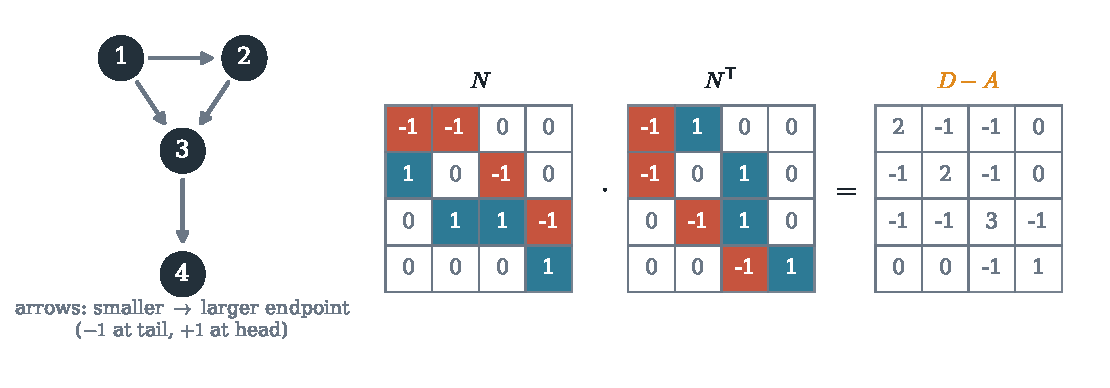
\includegraphics[width=0.98\textwidth]{mt_fig3_gram}
  \caption{El Teorema~\ref{thm:gram} sobre el grafo tri\'angulo-con-cola. Cada columna de $N$
  guarda el par $\pm1$ de una arista; la fila $u$ multiplicada por s\'i misma cuenta $(\pm1)^2$
  una vez por arista incidente (el grado), y multiplicada por la fila $w$ solo ve la arista
  com\'un, que aporta $-1$. Los signos son lo que fabrica el laplaciano: la matriz sin orientar
  dar\'ia $D+A$.}
  \label{fig:gram}
\end{figure}

La utilidad de la factorizaci\'on es que convierte hechos espectrales en contabilidad: la
semidefinici\'on positiva de $L$ es inmediata
($x^{\mathsf T}NN^{\mathsf T}x=\|N^{\mathsf T}x\|^2$ sobre $\R$), el n\'ucleo son las funciones
localmente constantes y---el uso que se hace aqu\'i---el determinante de cualquier submatriz
cuadrada de $L$ se vuelve una suma de Cauchy--Binet. En Lean la demostraci\'on es un c\'alculo
entrada a entrada: la diagonal eleva al cuadrado la fila de la incidencia sin orientar
(\lean{orientedIncMatrix\_mul\_self}), cuya suma Mathlib ya sabe que es el grado; el producto
extradiagonal de dos filas distintas se concentra en la arista com\'un, donde los signos son
opuestos por construcci\'on.

% ---------------------------------------------------------------
\section{Quitar la ra\'iz, elevar los menores al cuadrado}
\label{sec:sum}

El laplaciano en s\'i es singular, as\'i que la cuenta vive una supresi\'on m\'as abajo.
Fijada la ra\'iz $v_0$, escribimos $N_0$ para $N$ sin la fila de $v_0$ y $L_0$ para $L$ sin la
fila ni la columna de $v_0$. Restringir el Teorema~\ref{thm:gram} da
$L_0=N_0N_0^{\mathsf T}$, y ahora $N_0$ es un rect\'angulo de
$(n-1)\times\binom{|V|}{2}$: exactamente la silueta de Cauchy--Binet, con
$B=N_0^{\mathsf T}$ la traspuesta de $A=N_0$, de modo que cada sumando es el producto de un
menor por su propia traspuesta: un cuadrado.

\begin{theorem}[{\lean{SimpleGraph.det\_reducedLapMatrix\_eq\_sum\_sq}}]
\label{thm:sum}
\keyeq{\det L_0\;=\;\sum_{\substack{S\subseteq\mathrm{Sym}^2V\\ |S|=n-1}}
  \bigl(\det N_{0,S}\bigr)^{2}}
donde $N_{0,S}$ es el menor cuadrado de $N_0$ sobre las columnas $S$.
\end{theorem}

Conviene fijarse en el rango de la suma: \emph{todos} los subconjuntos de pares de v\'ertices
con $n-1$ elementos, sean aristas o no. Las columnas de los no-ejes son nulas, as\'i que sus
subconjuntos no aportan nada---pero est\'an honestamente dentro de la suma, y el enunciado
formal lo dice. Para $K_4$ la suma tiene $\binom{6}{3}=20$ t\'erminos; la Tabla~\ref{tab:k4}
los clasifica. El determinante se ha convertido en un \emph{censo}: el resto de la
demostraci\'on consiste en decidir, subconjunto a subconjunto, qui\'en contribuye.

\begin{table}[h]
\centering
\rowcolors{2}{ggband!35}{white}
\begin{tabular}{lccc}
\toprule
\rowcolor{ggteal!18} los 20 subconjuntos ($K_4$, $|S|=3$) & cu\'antos & $(\det N_{0,S})^2$ & aporte \\
\midrule
\'arboles generadores                      & 16 & 1 & 16 \\
tri\'angulos (4.\textsuperscript{o} v\'ertice aislado) & 4  & 0 & 0  \\
\bottomrule
\end{tabular}
\caption{El censo de $K_4$: todo subconjunto de 3 de sus 6 aristas o bien genera un \'arbol o
bien es uno de los cuatro tri\'angulos, que dejan un v\'ertice colgado. $\det L_0=16+0=16$, en
acuerdo con la Figura~\ref{fig:k4}. (Un subconjunto de 3 aristas sobre 4 v\'ertices deja de ser
\'arbol generador exactamente cuando es un tri\'angulo.)}
\label{tab:k4}
\end{table}

Una observaci\'on t\'ecnica, de las que una formalizaci\'on no puede despachar con un gesto:
Cauchy--Binet necesita un orden lineal sobre el tipo de columnas $\mathrm{Sym}^2V$ para nombrar
sus menores ordenados. No hay ninguno can\'onico, as\'i que el desarrollo instala uno con
alcance local---lexicogr\'afico sobre el par (extremo menor, extremo mayor)---como puro aparato
de indexaci\'on. A los determinantes al cuadrado no les importa qu\'e orden se eligi\'o, y el
enunciado del Teorema~\ref{thm:sum} cuantifica sobre subconjuntos, no sobre \'ordenes.

% ---------------------------------------------------------------
\section{Qu\'e menores sobreviven: ordenar en vez de inducir}
\label{sec:dichotomy}

\begin{theorem}[{\lean{SimpleGraph.sq\_det\_minor\_eq\_ite}}]
\label{thm:dichotomy}
Sea $R$ un dominio \'integro y $|S|=n-1$. Entonces
\keyeq{\bigl(\det N_{0,S}\bigr)^2\;=\;
\begin{cases}
  1 & \text{si } S\subseteq E(G)\ \text{y}\ (V,S)\ \text{es conexo,}\\[2pt]
  0 & \text{en caso contrario.}
\end{cases}}
\end{theorem}

Con $n-1$ aristas, ((conexo)) \emph{es} ((\'arbol generador)); el enunciado Lean usa la forma
con conexi\'on porque es la que consume la demostraci\'on, y un lema aparte la convierte en
\lean{IsTree} para el teorema principal (\lean{connected\_fromEdgeSet\_iff\_isTree}). La
demostraci\'on son tres casos, en orden creciente de inter\'es.

\emph{Un no-eje en $S$.} Su columna de $N_0$ es nula, y un determinante con una columna nula es
cero. Por aqu\'i se va tambi\'en la diagonal de $\mathrm{Sym}^2V$: un lazo $\{v,v\}$ no es
arista de un grafo simple, as\'i que los subconjuntos que contengan uno mueren en este caso.

\emph{Todo aristas, pero $(V,S)$ no conexo.} Alguna componente conexa $C$ no contiene la
ra\'iz. S\'umense las filas de $N_{0,S}$ sobre los v\'ertices de $C$: cada columna de una
arista interior a $C$ encuentra su $+1$ y su $-1$; ninguna arista de $S$ sale de $C$; el
resultado es la fila nula, exhibida en Lean como un vector no nulo del n\'ucleo de la
traspuesta (\lean{Matrix.exists\_vecMul\_eq\_zero\_iff}---este es el \'unico paso que pide un
dominio \'integro). Para los subconjuntos fallidos de la Tabla~\ref{tab:k4} la componente es un
solo v\'ertice colgado y la dependencia es simplemente ((su fila es nula)); en general $C$
puede ser mayor, y el trabajo lo hace el vector indicador de $C$.

\emph{Todo aristas, $(V,S)$ conexo.} Este es el caso que los libros de texto demuestran podando
una hoja e induciendo sobre $n$, y el caso en que la demostraci\'on formal hace otra cosa.

\begin{figure}[t]
  \centering
  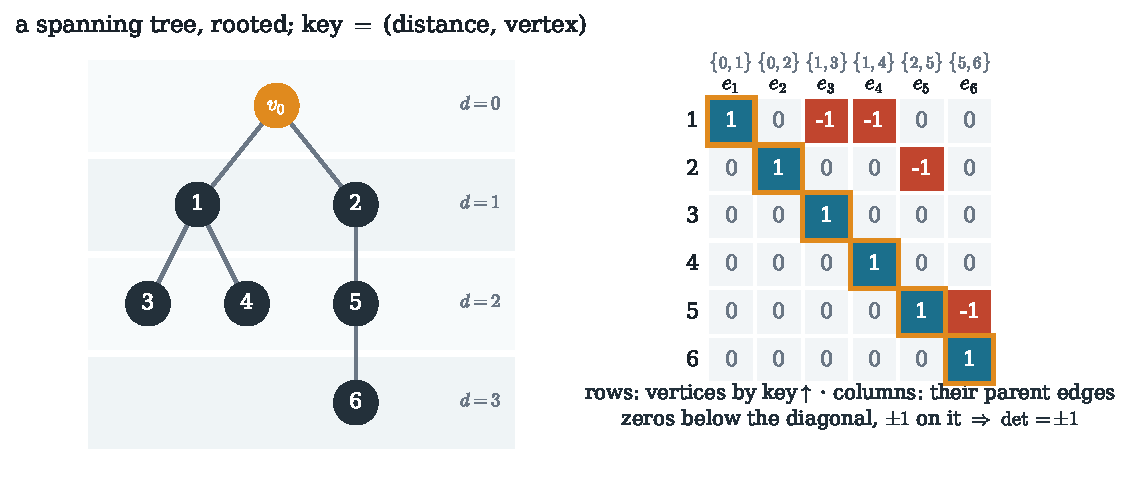
\includegraphics[width=0.97\textwidth]{mt_fig4_triangular}
  \caption{El caso conexo del Teorema~\ref{thm:dichotomy}. Izquierda: un \'arbol generador con
  ra\'iz $v_0$, v\'ertices con clave (distancia a la ra\'iz, v\'ertice). Derecha: el menor
  $N_{0,S}$ con la columna de cada v\'ertice elegida como su \emph{arista padre} y ambos lados
  ordenados por la clave. Un v\'ertice encuentra su propia arista padre en la diagonal ($\pm1$,
  enmarcada) y las aristas padre de sus hijos a la derecha (su clave es mayor); todo lo que
  queda bajo la diagonal se anula, y $\det=\pm1$ se lee de la diagonal.}
  \label{fig:triangular}
\end{figure}

Todo v\'ertice $u$ distinto de la ra\'iz de un subgrafo conexo tiene un vecino estrictamente
m\'as cercano a la ra\'iz: el segundo v\'ertice de cualquier geod\'esica de $u$ a $v_0$.
Llamemos \emph{arista padre} de $u$ a la arista hacia ese vecino. Dos hechos, ambos demostrados
con pura aritm\'etica de distancias:

\begin{itemize}
\item \emph{La aplicaci\'on $u\mapsto\text{arista padre de }u$ es inyectiva.} Si dos v\'ertices
compartieran arista padre en la forma cruzada ($u$ padre de $u'$ y $u'$ de $u$), sus distancias
a la ra\'iz cumplir\'ian $d(u)=d(u)+2$. Con $|S|=n-1$ y $n-1$ v\'ertices distintos de la
ra\'iz, inyectiva significa biyectiva: \emph{toda} arista de $S$ es arista padre de alguien.
\item \emph{Triangularidad.} Re-column\'ese el menor de modo que la columna del v\'ertice $u$
sea su arista padre, y ord\'enense filas y columnas por la clave $(\dist(u,v_0),u)$. Una entrada
no nula en la fila $u$, columna (arista padre de $w$), fuerza $u\in\{w,\text{padre de }w\}$: o
la diagonal, o $\dist(u,v_0)=\dist(w,v_0)-1$, clave estrictamente \emph{menor}. Todo lo que
queda bajo la diagonal es cero (Figura~\ref{fig:triangular}), las entradas diagonales son
$\pm1$ (cada v\'ertice est\'a sobre su propia arista padre), y $\det N_{0,S}=\pm1$.
\end{itemize}

En Lean, la re-columnaci\'on es un \lean{Equiv} construido con la inyectividad m\'as el conteo
de cardinales, la ordenaci\'on es \lean{Finset.orderIsoOfFin} aplicada a la imagen de la clave,
la anulaci\'on es \lean{Matrix.BlockTriangular} con \lean{Matrix.det\_of\_upperTriangular}, y
el signo se lava en el cuadrado. Merece la pena nombrar sin rodeos dos decisiones de
ingenier\'ia. \emph{Sin inducci\'on}: el orden lineal sobre las claves hace el trabajo que en
los libros hace la recursi\'on por poda de hojas, y una matriz ordenada es algo que un
asistente de demostraci\'on maneja con mucha m\'as gracia que una cirug\'ia de grafos.
\emph{Sin lema separado de aciclicidad}: la conexi\'on da a cada v\'ertice un padre y el
conteo hace sobreyectiva la aplicaci\'on, que es todo lo que el argumento necesita.
Matem\'aticamente no hay sorpresa---con $n-1$ aristas, conexi\'on y aciclicidad son
caracterizaciones equivalentes de los mismos \'arboles---pero en un desarrollo formal elegir
qu\'e caracterizaci\'on consumir es trabajo real ahorrado, y aqu\'i la mitad ac\'iclica nunca
tiene que materializarse.

% ---------------------------------------------------------------
\section{Verificaci\'on num\'erica}
\label{sec:verification}

Cada eslab\'on de la cadena se valid\'o num\'ericamente---en aritm\'etica exacta, nunca en coma
flotante---\emph{antes} de intentar su demostraci\'on Lean, y el enunciado ensamblado se
valid\'o de extremo a extremo despu\'es. La Tabla~\ref{tab:verification} lo resume.

\begin{table}[h]
\centering\footnotesize
\rowcolors{2}{ggband!35}{white}
\begin{tabular}{lll}
\toprule
\rowcolor{ggteal!18} comprobaci\'on & alcance & resultado \\
\midrule
enunciado de Cauchy--Binet, indexado ordenado & $2\times3\cdot3\times2$, exacto & coincide ($-264$) \\
menores de \'arboles: triangulares, $\det=\pm1$ & 200 \'arboles aleatorios, $n\le9$ & todos pasan \\
subconjuntos de $n{-}1$ aristas sin \'arbol: $\det=0$ & 158 grafos aleatorios & todos pasan \\
$(\det N_{0,S})^2=\mathbb 1[S$ genera \'arbol$]$, cada $S$ & 40 grafos, todos los $S$ & todos pasan \\
$\sum_S(\det N_{0,S})^2=\det L_0=\tau(G)$ & los mismos 40 grafos & todos pasan \\
grafos con nombre (Tabla~\ref{tab:numbers}) & 6 grafos & todos coinciden \\
\lean{\#print axioms}, los cinco teoremas & --- & 3 axiomas est\'andar \\
compilaci\'on completa de la biblioteca & \lean{lake build} & 3074 trabajos, sin errores \\
\bottomrule
\end{tabular}
\caption{La bater\'ia de verificaci\'on (SageMath 10, aritm\'etica entera exacta).}
\label{tab:verification}
\end{table}

\emph{Tama\~no y dependencias.} El desarrollo es peque\~no: $834$ l\'ineas de Lean en los
cinco ficheros de la Tabla~\ref{tab:loadbearing}, con $35$ declaraciones en total (teoremas,
lemas, dos definiciones y dos instancias locales), que importan once ficheros de Mathlib (el
n\'ucleo de \lean{SimpleGraph}, \lean{LapMatrix}, \lean{IncMatrix}, la m\'etrica de grafos, el
API de determinantes y matrices triangulares por bloques, y el orden de \lean{Sym2}). Con la
cach\'e de Mathlib v4.30 caliente, cada fichero se reverifica en $7$--$9$ segundos; la
compilaci\'on completa del proyecto (la biblioteca y todas las partes de la serie) son $3074$
trabajos.

De esta bater\'ia merece contarse un incidente, porque ense\~na al m\'etodo gan\'andose el pan.
El primer modelo num\'erico del menor colocaba entradas $\pm1$ en \emph{todas} las columnas,
no-ejes incluidos, y produjo de inmediato un contraejemplo al Teorema~\ref{thm:dichotomy}: una
estrella generadora cuyas aristas no pertenec\'ian todas al grafo segu\'ia teniendo
$\det=\pm1$. La discrepancia estaba en el modelo, no en las matem\'aticas---la
\lean{orientedIncMatrix} de Lean da a los no-ejes columnas \emph{nulas}, que es precisamente el
caso primero de la dicotom\'ia---y el modelo corregido pas\'o los $40$ grafos. Un arn\'es de
verificaci\'on que no puede cazar los errores de su propio operador es decoraci\'on; este
caz\'o el m\'io.

% ---------------------------------------------------------------
\section{La frontera: qu\'e est\'a demostrado y qu\'e no}
\label{sec:boundary}

\emph{Demostrado.} Los Teoremas~\ref{thm:cb}--\ref{thm:kirchhoff}, libres de \lean{sorry}, para
grafos simples finitos, cualquier ra\'iz, sobre cualquier dominio \'integro ($\Z$, $\mathbb Q$,
$\R$, \dots). Las cinco llamadas a \lean{\#print axioms} devuelven \lean{propext},
\lean{Classical.choice}, \lean{Quot.sound} y nada m\'as.

\emph{La hip\'otesis de dominio.} Los casos primero y tercero de la dicotom\'ia valen sobre
cualquier anillo conmutativo; el caso no conexo convierte un vector del n\'ucleo en un
determinante nulo, que es donde estorbar\'ian los divisores de cero. Como la igualdad principal
es entre un determinante y un n\'umero natural, demostrarla sobre $\Z$ (o $\mathbb Q$) y
transportarla no pierde nada; la hip\'otesis se declara con honestidad en lugar de esconderse.

\emph{Contar, no construir.} La demostraci\'on es no computable en el sentido de Lean: los
padres se eligen con \lean{Classical.choice} y no se extrae algoritmo alguno (ni de conteo ni
de muestreo). El determinante de la izquierda es, por supuesto, computable con cualquier
sistema de \'algebra lineal; el teorema es lo que \emph{justifica} ese c\'alculo.

\emph{No construido, cartografiado.} La versi\'on con pesos (el polinomio de Kirchhoff: dar a
cada arista una indeterminada y el determinante reducido enumera \'arboles por monomios) solo
necesita la misma cadena con entradas $\pm x_e$---el argumento triangular de la dicotom\'ia
pasa con $x_e$ en lugar de $\pm1$---pero no est\'a formalizada aqu\'i. Tampoco lo est\'an el
teorema de todos los menores~\cite{ChaikenKleitman1978}, la versi\'on dirigida (arborescencias,
\cite{Tutte1948}), ni la independencia de la ra\'iz como enunciado exento (aqu\'i es un
corolario: ambos lados cuentan los mismos \'arboles).

\emph{Trabajo previo, dicho con exactitud.} Sobre Cauchy--Binet: Mathlib no tiene versi\'on
alguna y, al escribir esto, ninguna pull request la menciona; existe una formalizaci\'on Lean
independiente en el proyecto que formaliza \emph{An Introduction to Algebraic Combinatorics} de
Grinberg~\cite{Grinberg,FaabianRepo}, con otra arquitectura de demostraci\'on (extracci\'on y
reconstrucci\'on expl\'icitas de la permutaci\'on, donde este desarrollo suma fibras y deja que
el determinante de $B$ se rearme solo). Ese proyecto es anterior a este; la versi\'on de
aqu\'i es independiente y se construy\'o para la cadena de arriba. Del teorema matricial de los
\'arboles en s\'i busqu\'e en el ecosistema Lean, en el Archive of Formal Proofs de Isabelle y
en el corpus Coq/Rocq, y no logr\'e localizar ninguna; hasta donde alcanza mi conocimiento no
la hay, y agradecer\'e cualquier correcci\'on.

% ---------------------------------------------------------------
\section{Implicaciones y metodolog\'ia}
\label{sec:implications}

\emph{D\'onde trabaja el teorema.} Tres consumidores, cada uno con la cantidad exacta que el
teorema suministra. \emph{Fiabilidad de redes}: $\tau(G)$ es el dato combinatorio principal del
polinomio de fiabilidad todos-los-terminales; comparar dise\~nos es comparar cuentas de
\'arboles generadores, y la Tabla~\ref{tab:numbers} es c\'omo se calculan. \emph{\'Arboles
generadores aleatorios}: el algoritmo de Wilson~\cite{Wilson1996} muestrea uniformemente entre
$\tau(G)$ \'arboles; el teorema de las corrientes de transferencia~\cite{BurtonPemantle1993}
hace determinantales las probabilidades de pertenencia de una arista---cocientes
$\tau(G/e)/\tau(G)$ de cuentas de \'arboles, es decir, resistencias efectivas.
\emph{Dispersi\'on espectral}: muestrear aristas por resistencia efectiva preserva el espectro
del laplaciano~\cite{SpielmanSrivastava2011}; la cantidad por la que se muestrea es, otra vez,
un cociente de los dos lados de este teorema. Ninguna de esas tuber\'ias est\'a formalizada
aqu\'i; lo formalizado es la identidad sobre la que todas se apoyan.

\emph{Para la biblioteca.} Dos piezas son candidatas naturales a Mathlib con independencia de
Kirchhoff: Cauchy--Binet (Secci\'on~\ref{sec:cb}) y la matriz de incidencia orientada con su
factorizaci\'on $NN^{\mathsf T}=D-A$ (Secci\'on~\ref{sec:gram}), que complementa la
\lean{incMatrix} sin orientar existente y su $D+A$. El argumento de la dicotom\'ia a\'isla
adem\'as un patr\'on reutilizable: \emph{sustituir la inducci\'on estructural por una
ordenaci\'on}---encontrar la clave inyectiva adecuada, y \lean{BlockTriangular} convierte una
recursi\'on de teor\'ia de grafos en la lectura de una diagonal.

\emph{Metodolog\'ia.} Como en las Partes~I--IV, la formalizaci\'on se llev\'o a cabo con un
asistente de IA (Claude, Anthropic) operando Lean contra un Mathlib local; el autor humano
fij\'o la direcci\'on, audit\'o cada afirmaci\'on y responde de cada enunciado. Las reglas de
trabajo no cambian y son breves: ((demostrado)) significa libre de \lean{sorry} con los axiomas
impresos; los dise\~nos se desriesgan num\'ericamente en aritm\'etica exacta antes de
formalizarse (Secci\'on~\ref{sec:verification}); las afirmaciones de novedad se contrastan con
la literatura y con los dem\'as ecosistemas de asistentes, y el trabajo previo
encontrado---aqu\'i, el Cauchy--Binet independiente de~\cite{FaabianRepo}---se informa en lugar
de omitirse.

% ---------------------------------------------------------------
\section{Preguntas que quedan abiertas}
\label{sec:questions}

Una formalizaci\'on es tambi\'en una lista de las siguientes preguntas, afiladas hasta que se
le puedan hacer a una m\'aquina.

\begin{itemize}
\item El argumento triangular lee $\det N_{0,S}=\pm1$ de una diagonal ordenada. El menor
\emph{con pesos}, con la indeterminada $x_e$ en lugar de $\pm1$, es triangular bajo la misma
clave, con diagonal $\pm\prod_{e\in S}$\,(un peso por arista padre). ?`Rinde el mismo esqueleto
de demostraci\'on el polinomio de Kirchhoff $\sum_T\prod_{e\in T}x_e$ cambiando solo la lectura
de la diagonal---y, en tal caso, ?`es el enunciado con pesos la generalidad correcta para
Mathlib desde el principio?
\item El caso no conexo necesita un dominio \'integro para convertir un vector del n\'ucleo en
$\det=0$. El determinante de una matriz con una componente sin ra\'iz es, de hecho, cero sobre
\emph{cualquier} anillo conmutativo (es una identidad entera). ?`Puede demostrarse la
dicotom\'ia con generalidad de anillo---por ejemplo exhibiendo la anulaci\'on como identidad
polin\'omica en las entradas---y suprimirse la hip\'otesis de dominio del
Teorema~\ref{thm:kirchhoff}?
\item ((Ordenar en vez de inducir)) funcion\'o porque la aplicaci\'on padre m\'as una clave
lineal volvieron triangular el menor. ?`Qu\'e otras inducciones sobre grafos son ordenaciones
encubiertas? El teorema de todos los menores~\cite{ChaikenKleitman1978} sustituye \'arboles por
bosques con varias ra\'ices---?`existe una clave multi-ra\'iz que triangularice esos menores de
una pasada?
\item Tanto este art\'iculo como la Parte~IV terminan en una identidad de determinantes cuya
demostraci\'on no toca jam\'as el objeto combinatorio que cuenta (all\'i, paseos cerrados;
aqu\'i, ciclos). ?`Hay una interfaz formal com\'un---((contar triangularizando un menor de
Gram))---bajo la cual los determinantes del lado de los emparejamientos y del lado de los
\'arboles sean instancias de un mismo lema?
\item El predicado \lean{Matrix.TotallyUnimodular} de Mathlib es exactamente ((todo menor
cuadrado vale $0$ o $\pm1$)). La dicotom\'ia demuestra una instancia af\'inada de \'el para
$N$. ?`Conectar\'ia registrar la unimodularidad total de $N$ este desarrollo con la parte de la
biblioteca de sabor optimizaci\'on, y da el argumento de la arista padre la demostraci\'on
m\'as corta de ese hecho?
\end{itemize}

Y una para guardar. \emph{Kirchhoff quer\'ia corrientes, y el determinante le entreg\'o unos
\'arboles que no hab\'ia pedido; la demostraci\'on de arriba no mira un ciclo ni una sola vez
y, sin embargo, termina sabiendo exactamente de cu\'antas maneras el grafo los evita todos.
?`Cu\'anto m\'as sabe ya una biblioteca capaz de tomar determinantes, que sencillamente
todav\'ia no dice?}

% ---------------------------------------------------------------
\begin{thebibliography}{99}

% --- las dos memorias de 1812 ---
\bibitem{Binet1812} J.~P.~M. Binet, \emph{M\'emoire sur un syst\`eme de formules analytiques,
et leur application \`a des consid\'erations g\'eom\'etriques}, J.~\'Ec.\ Polytech.\
\textbf{9}, cahier~16 (1813), 280--354. Le\'ida el 30 de noviembre de 1812.
\bibitem{Cauchy1812} A.-L. Cauchy, \emph{M\'emoire sur les fonctions qui ne peuvent obtenir que
deux valeurs \'egales et de signes contraires par suite des transpositions op\'er\'ees entre
les variables qu'elles renferment}, J.~\'Ec.\ Polytech.\ \textbf{10}, cahier~17 (1815),
29--112. Le\'ida el 30 de noviembre de 1812.

% --- el teorema matricial de los arboles: origen y demostraciones clasicas ---
\bibitem{Kirchhoff1847} G.~Kirchhoff, \emph{\"Uber die Aufl\"osung der Gleichungen, auf welche
man bei der Untersuchung der linearen Vertheilung galvanischer Str\"ome gef\"uhrt wird},
Ann.\ Phys.\ Chem.\ \textbf{72} (1847), 497--508.
\bibitem{Borchardt1860} C.~W. Borchardt, \emph{\"Uber eine Interpolationsformel f\"ur eine Art
symmetrischer Functionen und \"uber deren Anwendung}, Abh.\ K\"onigl.\ Akad.\ Wiss.\ Berlin
(1860), 1--20.
\bibitem{Cayley1889} A.~Cayley, \emph{A theorem on trees}, Quart.\ J.~Pure Appl.\ Math.\
\textbf{23} (1889), 376--378.
\bibitem{BSST1940} R.~L. Brooks, C.~A.~B. Smith, A.~H. Stone, and W.~T. Tutte, \emph{The
dissection of rectangles into squares}, Duke Math.\ J.~\textbf{7} (1940), 312--340.
\bibitem{Tutte1948} W.~T. Tutte, \emph{The dissection of equilateral triangles into equilateral
triangles}, Proc.\ Cambridge Philos.\ Soc.\ \textbf{44} (1948), 463--482.
\bibitem{ChaikenKleitman1978} S.~Chaiken and D.~J. Kleitman, \emph{Matrix tree theorems},
J.~Combin.\ Theory Ser.~A \textbf{24} (1978), 377--381.
\bibitem{Chaiken1982} S.~Chaiken, \emph{A combinatorial proof of the all minors matrix tree
theorem}, SIAM J.~Algebraic Discrete Methods \textbf{3} (1982), 319--329.

% --- referencias clasicas ---
\bibitem{Moon1970} J.~W. Moon, \emph{Counting Labelled Trees}, Canadian Math.\ Monographs
\textbf{1}, Canadian Math.\ Congress, 1970.
\bibitem{Biggs1993} N.~Biggs, \emph{Algebraic Graph Theory}, 2.\textsuperscript{a} ed.,
Cambridge Univ.\ Press, 1993.
\bibitem{GodsilRoyle} C.~Godsil and G.~Royle, \emph{Algebraic Graph Theory}, Grad.\ Texts in
Math.\ \textbf{207}, Springer, 2001.
\bibitem{StanleyEC2} R.~P. Stanley, \emph{Enumerative Combinatorics, Volume~2}, Cambridge
Stud.\ Adv.\ Math.\ \textbf{62}, Cambridge Univ.\ Press, 1999.

% --- probabilidad y algoritmos modernos sobre arboles generadores ---
\bibitem{Wilson1996} D.~B. Wilson, \emph{Generating random spanning trees more quickly than the
cover time}, en \emph{Proc.\ 28th ACM Symp.\ Theory of Computing} (STOC~1996), 296--303.
\bibitem{BurtonPemantle1993} R.~Burton and R.~Pemantle, \emph{Local characteristics, entropy
and limit theorems for spanning trees and domino tilings via transfer-impedances}, Ann.\
Probab.\ \textbf{21} (1993), 1329--1371.
\bibitem{SpielmanSrivastava2011} D.~A. Spielman and N.~Srivastava, \emph{Graph sparsification
by effective resistances}, SIAM J.~Comput.\ \textbf{40} (2011), 1913--1926.
\bibitem{LyonsPeres} R.~Lyons and Y.~Peres, \emph{Probability on Trees and Networks}, Cambridge
Univ.\ Press, 2016.

% --- contexto de formalizacion ---
\bibitem{Grinberg} D.~Grinberg, \emph{An Introduction to Algebraic Combinatorics}, notas de
curso, 2026. \texttt{arXiv:2506.00738}.
\bibitem{FaabianRepo} \emph{algebraic-combinatorics: una formalizaci\'on en Lean~4 de ``An
Introduction to Algebraic Combinatorics'' de Grinberg},
\url{https://github.com/faabian/algebraic-combinatorics}, 2026. Cauchy--Binet en el blueprint,
\S5.2.
\bibitem{Mathlib} The mathlib Community, \emph{The Lean mathematical library}, en \emph{Proc.\
9th ACM SIGPLAN Int.\ Conf.\ on Certified Programs and Proofs} (CPP~2020), 367--381.

% --- esta serie ---
\bibitem{PartI} C.~Mar\'in, \emph{Random Signs into Matchings: the Godsil--Gutman estimator and
real-rootedness in Lean~4} (Parte~I), 2026. Zenodo, DOI \texttt{10.5281/zenodo.20517350}.
\bibitem{PartII} C.~Mar\'in, \emph{Unfolding a Graph into a Tree: A Machine-Checked Proof of
the Heilmann--Lieb Theorem in Lean~4} (Parte~II), 2026. Zenodo, DOI
\texttt{10.5281/zenodo.20561832}.
\bibitem{Bass} C.~Mar\'in, \emph{Folding Edges into Vertices: A Machine-Checked Proof of Bass's
Determinant Formula for the Ihara Zeta in Lean~4}, 2026. Zenodo, DOI
\texttt{10.5281/zenodo.20573120}.
\bibitem{PartIII} C.~Mar\'in, \emph{Walks that Forget the Cycles: A Machine-Checked Bijection
between Tree-Like Walks of a Graph and Walks on Godsil's Path Tree, in Lean~4} (Parte~III),
2026. Zenodo, DOI \texttt{10.5281/zenodo.20600326}.
\bibitem{PartIV} C.~Mar\'in, \emph{When Walks Become a Spectrum: A Machine-Checked Proof of
Godsil's Moment Theorem in Lean~4} (Parte~IV), 2026. Zenodo, DOI
\texttt{10.5281/zenodo.20613247}.

\end{thebibliography}

\end{document}
